%%%%%%%%%%%%%%%%%%%%%%%%%%%%%%%%%%%%%%%%%%%%%%%%%%%%%%%%%%%%%%%%%%%%%%%%%%
%% Trim Size: 10.25in x 7.5in            %Raj - 09 Feb 2004
%% Text Area: 8.5in (include Runningheads) x 6in
%% ws-jca.tex   :  23-5-2008
%% Tex file to use with ws-jca.cls written in Latex2E.
%%%%%%%%%%%%%%%%%%%%%%%%%%%%%%%%%%%%%%%%%%%%%%%%%%%%%%%%%%%%%%%%%%%%%%%%%%%%

\documentclass{ws-jca}
\usepackage{graphicx} 
\newcommand{\threeD}{3\nobreakdash\textendash D }	% for "3-D'' with no break
\newcommand{\twoD}{2\nobreakdash\textendash D }	% for "2-D'' with no break
\newcommand{\twoDxN}{2\nobreakdash\textendash DxN }
\newcommand{\Cerveny}{\v{C}erven\'{y} }
% \newcommand{\deg}{\textsuperscript{o}}

\renewcommand{\thefootnote}{\fnsymbol{footnote}}

\begin{document}

\markboth{S. M. Reilly, G. Potty}
{Hybrid Gaussian Beams in Spherical/Time Coordinates}

%%%%%%%%%%%%%%%%%%%%% Publisher's Area please ignore %%%%%%%%%%%%%%%
%
\catchline{}{}{}{}{}
%
%%%%%%%%%%%%%%%%%%%%%%%%%%%%%%%%%%%%%%%%%%%%%%%%%%%%%%%%%%%%%%%%%%%%

\title{Sonar Propagation Modeling using Hybrid Gaussian Beams in Spherical/Time Coordinates}

\author{Sean M. Reilly}
\address{Department of Ocean Engineering, University of Rhode Island,\\
Narragansett RI, USA\\
\email{campreilly@my.uri.edu} }

\author{Gopu Potty}
\address{Department of Ocean Engineering, University of Rhode Island,\\
Narragansett RI, USA\\
\email{potty@egr.uri.edu} }

\maketitle

\begin{history}
\received{(Day Month Year)}
\revised{(10 January 2012)}
\end{history}

\begin{abstract}
This paper defines a new \threeD underwater acoustic propagation loss model that is
specifically formulated to provide a significant speed advantage to real-time, active sonar, simulation/stimulation systems in littoral environments.  The ray
solutions to the eikonal equation are computed in latitude, longitude, and
altitude coordinates to match wide-area environmental databases. Hybrid
Gaussian beam techniques for propagation loss calculation are used to
extend the applicability of ray theory to lower frequency regimes.
Numerical integration of the wave equation is performed in the time
dimension to maintain the phase continuity of the wavefront. This \threeD
approach supports horizontal refraction and 
out-of-plane reflection from the ocean bottom. 
Computing the transmission loss in the same coordinate system as the
environmental parameters should provide this model with a computational
speed advantage over other models. The derivation of this new model
requires the development of new equations for ray tracing, reflection,
eigenray finding, and Gaussian beam propagation loss. This paper examines
that derivation.
\end{abstract}

\keywords{Gaussian beams; \threeD modeling; range-dependent; time-domain.}

\section{Introduction}

Ray models are one of the oldest techniques for understanding sound
propagation in the ocean. Although much of the current literature focuses
on full-wave methods, such as normal mode and parabolic equation,
range-dependent ray theory is still used frequently by real-time sonar
simulation/stimulation systems to compute propagation loss. This is partly
due to the fact that ray models run quickly, and partly because they provide the travel
time and direction information needed for sonar stimulation. This
preference is particularly acute at higher frequencies (above 1000 Hz),
where full-wave methods become prohibitively slow.  Unfortunately, ray models
can also suffer from significant accuracy limitations: they predict perfect 
shadow zones in areas of the water column where rays do not propagate, 
and they predict infinite intensity at
caustics, places where the ray paths cross.\cite{Baxley2000} These effects
are not seen in nature and full-wave models do not suffer from these
problems.  Gaussian beams are an augmentation of ray theory that attempts to address
these limitations while keeping many of ray theory's benefits. This paper
builds on the prior art in Gaussian beam theory 
to create a new propagation loss model that
operates in a fully \threeD environment. Future papers will focus on the
verification, validation, and computational efficiency of this new model.

The Gaussian beam components of this new approach leverage the concepts
developed by H. Weinberg et. al.\cite{Weinberg1996,GRAB2008} for the Gaussian Ray
Bundling (GRAB) model. Gaussian beam models compute propagation
loss by spreading the energy associated with each ray path, across the wavefront, 
out to a distance that is proportional to the divergence of the acoustic
field along this path. The propagation loss for each target is computed by
summing the contributions from many passing rays. This enhancement
eliminates the tendency toward infinite intensity at caustics, and it
produces penetration into shadow zones, especially at low frequencies.

In 1982, V. \Cerveny et. al.\cite {Cerveny1982} developed a rigorous method for
computing seismic Gaussian beams. \v{C}erven\'{y}'s approach uses dynamic ray
equations to compute the divergence of the field along the ray path. In
1987, M. B. Porter et. al.\cite{Porter1994,Porter1987} extended this work to underwater
acoustics and created the BELLHOP\footnote{BELLHOP is not an acronym.}
model. GRAB (1996) leverages this prior work,
but calculates the divergence using the distance between ray paths, much
like classic ray theory. The fact that GRAB does not need to compute and
maintain the dynamic ray equations, gives it a speed advantage over these
other methods. In general, Gaussian
beam propagation loss calculations are expected to be most accurate at
frequencies above 1000 Hz, but GRAB has successfully used these techniques
to support accurate results at frequencies as low as 150 Hz. Because GRAB
combines Gaussian beams with traditional ray theory, it is sometimes
categorized as a ``hybrid'' Gaussian beam model. All of these models are based
on a Cartesian \twoD coordinate system and they use multiple radials to
model \threeD effects. This process is often referred to as a \twoDxN
approach.

The new algorithm uses geographic latitude, longitude, and altitude as the
basis for a \threeD propagation environment. This approach is very similar to the one
developed by R. M. Jones et. al.\cite{Jones1986} for the Hamiltonian
Ray-Tracing Program for the Ocean (HARPO). This coordinate system not only
supports horizontal refraction, and out-of-plane reflection, but also allows ray
tracing to be performed in the same coordinate system as environmental
parameter databases. Most ray theory models, including all of the models
referenced above, are based on solutions to the eikonal equation, the high
frequency limit of Helmholtz equation. The HARPO model is unusual in that it
solves the Hamilton equation, the differential expression of Fermat's
principle, using an elliptical earth. This difference gives HARPO the
ability to model the frequency spreading effects associated with ocean
advection on planetary scales. However, at this time, HARPO only computes ray
paths, not propagation loss.

This paper combines all of these concepts into a new propagation loss algorithm that is
specifically formulated to provide a significant speed advantage to real-time, active sonar, simulation/stimulation systems in littoral environments.  It solves
the eikonal ray tracing equations as functions of geographic latitude,
longitude, and altitude. The earth is modeled
as a sphere, with a radius that depends on the area of operations, instead
of using HARPO's elliptical representation, to simplify this computation,  
Although there are increased
computational requirements for modeling Gaussian beams in this
coordinate system, the impact on calculation speed is 
balanced by the ability to compute solutions
without transforming environmental parameter databases into \twoDxN radials.
Numerical integration of the ray equations is performed in the time
dimension to maintain the phase continuity of the wavefront, which
simplifies the eigenray finding geometry. Propagation loss is calculated
using a technique that is similar to GRAB, but translated into a new \threeD coordinate system. The derivation of this new approach requires
the development of new equations for ray tracing, reflection, eigenray
finding, and Gaussian beam propagation loss. This paper examines
that derivation.

\section{Ray Tracing in Spherical/Time Coordinates}

The ray tracing equations used by this model are

\begin{equation}
	\frac{dr}{dt} = c^2 \alpha \:,
	\label{eq:dr_dt}
\end{equation}
\begin{equation}
	\frac{d\theta}{dt} = \frac{c^2 \beta}{r} \:,
	\label{eq:dtheta_dt}
\end{equation}
\begin{equation}
	\frac{d\phi}{dt} = \frac{c^2\gamma}{r sin\theta} \:,
	\label{eq:dphi_dt}
\end{equation}
\begin{equation}
	\frac{d\alpha}{dt} = -\frac{1}{c}\frac{dc}{dr} 
		+ \frac{c^2}{r}\left( \beta^2 + \gamma^2 \right) \:,
	\label{eq:dalpha_dt}
\end{equation}
\begin{equation}
	\frac{d\beta}{dt} = -\frac{1}{cr}\frac{dc}{d\theta} 
		- \frac{c^2 \alpha \beta}{r} + \gamma^2 cot\theta \:,
	\label{eq:dbeta_dt}
\end{equation}
\begin{equation}
	\frac{d\gamma}{dt} = -\frac{1}{cr sin\theta}\frac{dc}{d\phi} 
		- \frac{c^2 \gamma}{r} \left( \alpha + \beta cot\theta \right) \:,
	\label{eq:dgamma_dt}
\end{equation}
where 
$c$ is the speed of sound in water; 
$t$ is the travel time along the ray path;
\((r,\theta,\phi)\) are the spherical components of \(\vec{r}\), the position along a ray path; and
\((\alpha,\beta,\gamma)\) are the spherical components of \(\vec{\xi}\), the propagation direction divided by the speed of sound.
Equations (\ref{eq:dr_dt}) through (\ref{eq:dgamma_dt}) compute the time
evolution for the location and direction for any acoustic ray based on its
initial conditions. These equations are derived from first principles in
Appendix A. These equations support \threeD refraction effects and
incorporate earth curvature effects, including great circle routes between
locations. Environmental parameters and their derivatives are computed
directly in geographic latitude, longitude, and altitude without reducing
the problem to a series of \twoDxN radials or a flat earth Cartesian
projection.

This model uses an explicit, third order, Adams-Bashforth (AB3)
algorithm\cite{Yakowitz1986} to propagate Eqs.~(\ref{eq:dr_dt}) through
(\ref{eq:dgamma_dt}) numerically. The AB3 algorithm, summarized in
Eq.~(\ref{eq:AB3_algorithm}), approximates each step in the solution for
f(\(t\)) using explicit information from the three time steps that
came before it. Since these past values can be cached, AB3 is much faster
than other methods with similar accuracy. However, because AB3 is not self-starting,
this model uses a third order Runge-Kutta (RK3) algorithm\cite{Press1992}
whenever the ray parameters must be initialized, or re-initialized
\begin{equation}
	f(t_{n+1}) = f(t_{n}) + \delta t \left[ 
		\frac{23}{12} \frac{df}{dt}(t_n)
	  	- \frac{16}{12} \frac{df}{dt}(t_{n-1}) 
	  	+ \frac{5}{12} \frac{df}{dt}(t_{n-2}) \right] \:.
	\label{eq:AB3_algorithm}
\end{equation}

Even though Eqs. (\ref{eq:dr_dt}) through (\ref{eq:dgamma_dt}) look complex, the ray tracing is still expected to be more computationally efficient than
an equivalent \twoDxN calculation in Cartesian coordinates. Most of these savings
are a result of the fact that this model avoids transformation of the
environmental inputs. 
These savings will be most significant in highly dynamic \threeD simulation
environments where the re-use of pre-computed environments is not
practical. It is helped by the fact that the interpolation of
the speed of sound and its gradient, an expensive operation for gridded
databases, have been limited to a single instance per iteration. In
addition, the computationally expensive trigonometric calculations have
been reduced to a single \(sin\theta\) and \(cot\theta\) factor per iteration.

\section{Boundary Reflections on a Spherical Earth}

\begin{figure}[th]
	\centerline{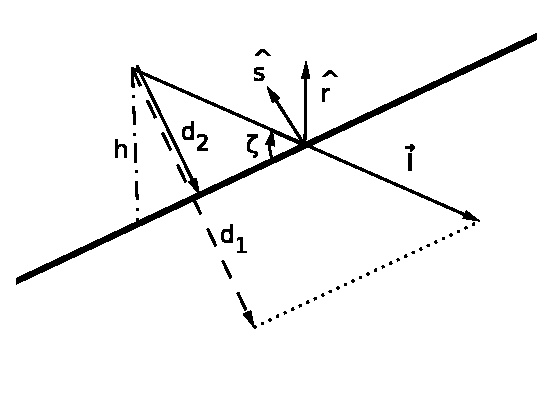
\includegraphics[width=3in]{EstPointCollision.eps}} 
	\vspace*{8pt}
	\caption{Estimating the point of reflection. }
	\label{fig:reflection_time}
\end{figure}

The first step in modeling an interface reflection is estimating the point in time when the incident ray strikes the bottom.  The derivation of the equations for estimating the time of reflection in spherical coordinates uses the symbols defined in Fig.~\ref{fig:reflection_time} where
\(\vec{I}\) is the incident ray path;
\(\zeta\) is the incident grazing angle;
\(\hat{s}\) is the surface normal;
\(\hat{r}\) is the unit vector in the radial direction;
\(h\) is the incident ray height above bottom;
\(\Delta t\) is the normal time step; and
\(\delta t\) is the time step needed to reach the interface.

If the bottom slope is nearly constant across the length of the incident
ray, then the ratio of the time steps is equivalent to the ratio of the
distances normal to the surface
\begin{equation}
	d_1 \equiv - \vec{I} \cdot \hat{s} 
		= - \left( \frac{d\vec{r}}{dt} \cdot \hat{s} \right) \Delta t \:,
	\label{eq:reflection_d1}
\end{equation}
\begin{equation}
	d_2 \equiv - h \hat{r} \cdot \hat{s} \:,
	\label{eq:reflection_d2}
\end{equation}
\begin{equation}
	\frac{\delta t}{\Delta t} = \frac{d_2}{d_1} 
		= \cfrac{h \: \hat{r} \cdot \hat{s}}{\left( \cfrac{d\vec{r}}{dt} 
		\cdot \hat{s} \right) \Delta t} \:,
	\label{eq:reflection_ratio}
\end{equation}
\begin{equation}
	\delta t = \cfrac{h \: \hat{r} \cdot \hat{s}}{\cfrac{d\vec{r}}{dt} \cdot \hat{s}} \:.
	\label{eq:reflection_time_bottom}
\end{equation}
At the ocean surface, this simplifies to
\begin{equation}
	\delta t_{surface} = \frac{h}{\frac{dr}{dt}} \:,
	\label{eq:reflection_time_surface}
\end{equation}
where \(\frac{dr}{dt}\) is the radial ray tracing component defined in
Eq.~(\ref{eq:dr_dt}).
To improve the accuracy of the reflection geometry, the new model also
applies a second order Taylor expansion to each component of the position,
normalized direction, and sound speed, to find their values at the point
defined by Eq. (\ref{eq:reflection_ratio}).

\begin{figure}[th]
	\centerline{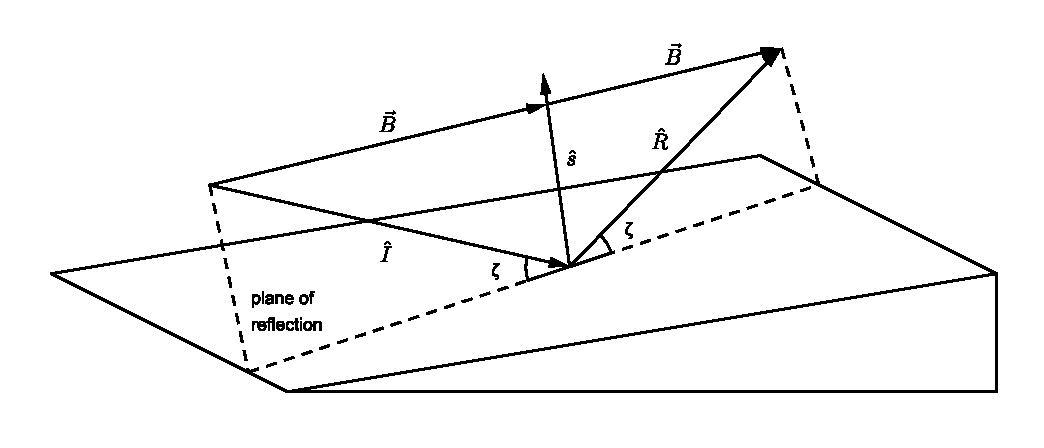
\includegraphics[width=3in]{EstDirectionCollision.eps}} 
	\vspace*{8pt}
	\caption{Reflection from a \threeD slope.}
	\label{fig:reflect3d}
\end{figure}
The next step in reflection modeling is estimating the direction of
reflection from a \threeD slope. The derivation of the equations for
estimating this direction in spherical coordinates uses the
symbols defined in Fig.~\ref{fig:reflect3d} 
where
\(\hat{I}\) is the incident ray path direction;
\(\hat{R}\) is the reflected ray path direction; and
\(\vec{B}\) is the component of the incident ray that is perpendicular to surface normal.

Since the reflected ray has the same angle to the normal as the incident ray
\begin{equation}
\hat{R} = 2\vec{B} - \hat{I} \:,
\label{eq:reflect_r_hat}
\end{equation}
\begin{equation}
\vec{B} =  \hat{I} - ( \hat{I} \cdot \hat{s} ) \hat{s} \:,
\label{eq:reflect_p_hat}
\end{equation}
\begin{equation}
\hat{R} =  \hat{I} - 2 ( \hat{I} \cdot \hat{s} ) \hat{s} \:.
\label{eq:reflect_direction}
\end{equation}
For ocean surface reflections, these relationships negate the sign of the
radial component while leaving the \(\theta\) and \(\phi\) direction
components unchanged.

Most bottom depth databases grid the relief of the earth's surface into a
series of geographic latitude and longitude points. The spherical components of the
surface normal (\( s_r, s_\theta, s_\phi\)) are computed by equating the
slope (\(\sigma_\theta, \sigma_\phi\)) to the first derivative of $b$, the
boundary altitude.
\begin{equation}
	\Omega_\theta \equiv tan(\sigma_\theta) 
		= \frac{1}{b} \frac{db}{d\theta} \:,
	\label{eq:slope_theta}
\end{equation}
\begin{equation}
	\Omega_\phi \equiv tan(\sigma_\phi) 
		= \frac{1}{b \: sin\theta} \frac{db}{d\phi} \:,
	\label{eq:slope_phi}
\end{equation}
\begin{equation}
	s_\theta = - sin(\sigma_\theta) 
		= -\frac{\Omega_\theta}{ \sqrt{1+\Omega^2_\theta} } \:,
	\label{eq:normal_theta}
\end{equation}
\begin{equation}
	s_\phi = - sin(\sigma_\phi) 
		= -\frac{\Omega_\phi}{ \sqrt{1+\Omega^2_\phi} } \:,
	\label{eq:normal_phi}
\end{equation}
\begin{equation}
	s_r = \sqrt{ 1- ( s^2_\theta + s^2_\phi )} \:.
	\label{eq:normal_r}
\end{equation}

After reflection, the ray must be reinitialized in a way that maintains the
phase continuity of the wavefront. This model uses a third order
Runge-Kutta (RK3) algorithm to reverse propagation from the point of
reflection back to the \(t_n\), \(t_{n-1}\), \(t_{n-2}\) points in time, during reinitialization.

\begin{figure}[th]
	\centerline{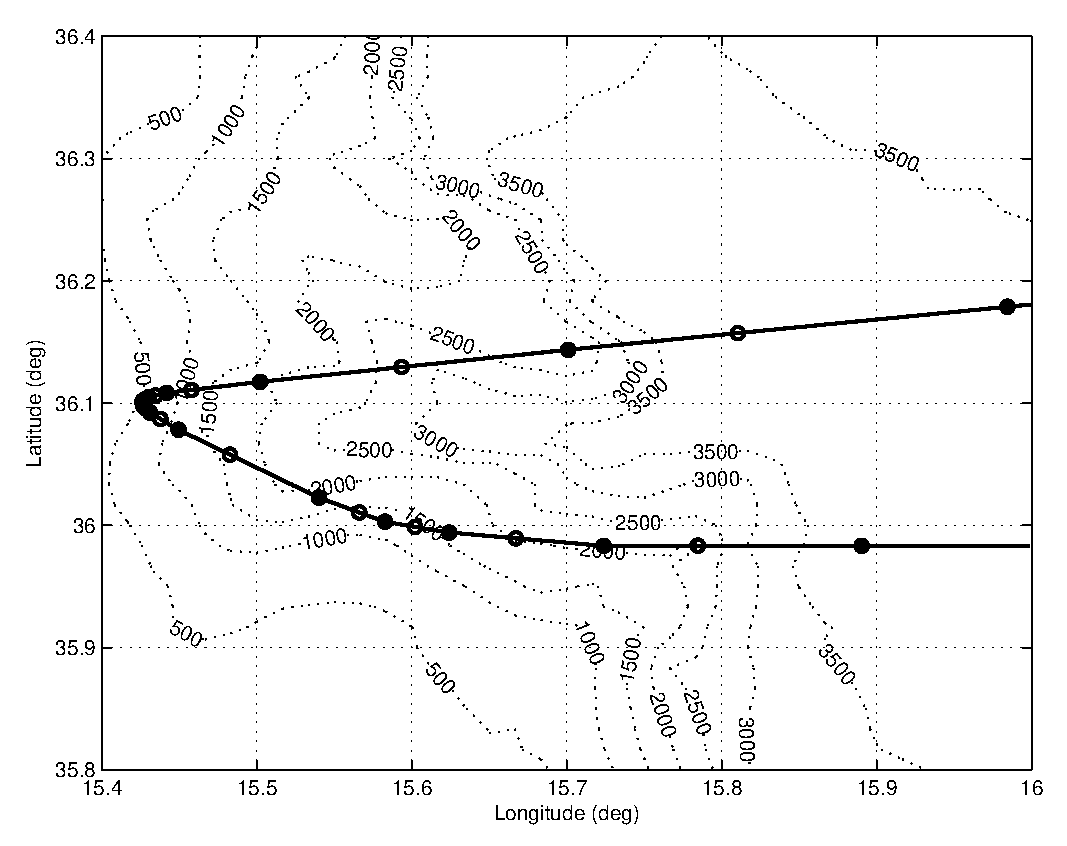
\includegraphics[width=4in]{reflect_grid_malta.eps}} 
	\vspace*{8pt}
	\caption{3-D Reflection on the Malta Escarpment.
	\label{fig:reflect_grid_malta}}
\end{figure}

ETOPO1 gridded bathymetry\cite{ETOPO1} from the Malta Escarpment was used
to test out-of-plane reflection from real world bathymetry features. The
results of this test are shown in Fig.~\ref{fig:reflect_grid_malta}. In
this Fig., bottom bathymetry contours are represented as dashed lines. A
ray is launched from 35:59N 16:00E, at a depth of 10 meters, with a
depression/elevation angle of -20\textsuperscript{o} (down), and an azimuth
of 270\textsuperscript{o}. The solid black line follows the trajectory of
the ray as a function of latitude and longitude. The open circles along
this path represent places where surface reflections occurred; the closed
circles represent bottom reflections. The speed of sound was artificially
fixed at 1500~m/s, and a time step of 100~ms was used to compute ray paths.
The decrease in spacing between the shallow water dots illustrates an
increase in the ray's depression/elevation angle as it reflects up the slope. In addition,
ray paths were reflected into a new azimuthal direction each time that they
interacted with the bottom. These out-of-plane reflections result in a down
slope ray path that is offset by more than 21.9 km from the up slope path,
after 14 bounces off of the bottom. This type of out of plane reflection is
exactly the type of behaviors that we would expect from real-world
bathymetry.\cite{Sturm2008}

\section{Finding Eigenrays using Coherent Wavefronts}

In this model, eigenrays are derived from each target's geometry relative
to a Closest Point of Approach (CPA) on the wavefront. A point on the
wavefront is the CPA for a specific target if the distance to that target
is less than the same measurement in the twenty-six wavefront points that
surround it. The coordinates for this distance calculation are illustrated
in Fig.~\ref{fig:eigenray_geometry}
where
\(\vec{r}_{p}\) is the position of the eigenray target;
\(\vec{r}_{njk}\) is the position of the candidate points on the wavefront;
\(d_{njk}\) is the distance from target to each point on wavefront;
\(\delta t\) is the target offset along the direction of propagation;
\(\delta\mu\) is the target offset in the depression/elevation direction; and 
\(\delta\varphi\) is the target offset in the azimuthal direction.
\begin{figure}[th]
	\centerline{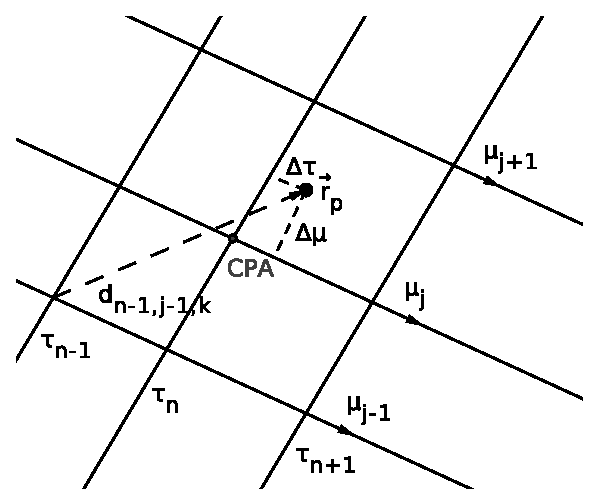
\includegraphics[width=3in]{EigenrayGeometry.eps}} 
	\vspace*{8pt}
	\caption{Eigenray estimation geometry 
		(side view: \(\varphi_k\) direction not shown).}
	\label{fig:eigenray_geometry}
\end{figure}

An efficient calculation for the square of the distance in spherical
coordinates can be derived from the Haversine formula\cite{Sinnott1984}
\begin{equation}
	d^2_{njk} = r^2_{p} + r^2_{njk} - 2 \vec{r}_{p} \cdot \vec{r}_{njk} \:,
	\label{eq:pythagoras1}
\end{equation}
\begin{equation}
	d^2_{njk} = r^2_{p} + r^2_{njk} - 2 r_{p} r_{njk}
	\left[ sin(\chi_{p}) sin(\chi_{ijk})
	+ cos(\chi_{p}) cos(\chi_{ijk}) cos(\phi_{p}-\phi_{ijk}) \right] \:,
	\label{eq:pythagoras2}
\end{equation}
\begin{align}
	d^2_{njk} &= r^2_{p} + r^2_{njk} - 2 r_{p} r_{njk}
	\left[ 1 - 2 \left\{ sin^2 \left( \frac{\chi_{p}-\chi_{ijk}}{2} \right) 
		\right.\right.\nonumber\\
	&\left.\left. {} + cos(\chi_{p}) cos(\chi_{ijk}) sin^2 
		\left( \frac{\phi_{p}-\phi_{ijk}}{2} \right) \right\} \right] \:,
\label{eq:haversine1}
\end{align}
\begin{align}
	d^2_{njk} &\approx r^2_{p} + r^2_{njk} - 2 r_{p} r_{njk}
	\left[ 1 - 2 \left\{ \left( \frac{\chi_{p}-\chi_{ijk}}{2} \right)^2 
		\right.\right.\nonumber\\
	&\left.\left. {} + cos(\chi_{p}) cos(\chi_{ijk}) 
		\left( \frac{\phi_{p}-\phi_{ijk}}{2} \right)^2 \right\} \right] \:,
	\label{eq:haversine2}
\end{align}
\begin{equation}
	d^2_{njk} \approx r^2_{p} + r^2_{njk} - 2 r_{p} r_{njk}
	\left[ 1 - 2 \left\{ \left( \frac{\theta_{p}-\theta_{ijk}}{2} \right)^2
		+ sin(\theta_{p}) sin(\theta_{ijk}) 
		\left( \frac{\phi_{p}-\phi_{ijk}}{2} \right)^2 \right\} \right] \:.
	\label{eq:haversine3}
\end{equation}

The accuracy of this approximation improves as the distance between the
target and the wavefront decreases. If the implementation caches values for
\(sin\theta\) at both the wavefront and target locations,
Eq.~(\ref{eq:haversine3}) allows \(d^2_{njk}\) to be computed without the
use of any additional transcendental functions.

The offset of each target relative to the travel time  (\(t\)),
depression/elevation launch angle (\(\mu\)), and the azimuthal launch
angle (\(\varphi\)) coordinates of the CPA are needed to compute eigenrays.
This model calculates these offsets by expressing \(d^2_{p}\), the square
of the distance at the target point, as a second
order Taylor series, in vector form, relative to the CPA
\begin{equation}
	\vec{\rho} \equiv (\rho_1, \rho_2, \rho_3) 
		\equiv (\delta t, \delta \mu, \delta \varphi) \:,
	\label{eq:rho_defined}
\end{equation}
\begin{equation}
	d^2_{p} \approx \epsilon + \vec{g} \cdot \vec{\rho} 
		+ \frac{1}{2} \vec{\rho} \cdot \mathbf{H} \: \vec{\rho} \:,
	\label{eq:taylor1}
\end{equation}
\begin{equation}
	\epsilon  \equiv d^2 \big|_{CPA} \:,
	\label{eq:taylor2}
\end{equation}
\begin{equation}
	\vec{g} \equiv \frac{\partial d^2}{\partial \vec{\rho} } \big|_{CPA} \:,
	\label{eq:taylor3}
\end{equation}
\begin{equation}
	\mathbf{H} \equiv \frac{\partial^2 d^2}{\partial \vec{\rho}^2 } \big|_{CPA}
	\label{eq:taylor4}
\end{equation}
where 
\(\vec{\rho}\) is the target offset from CPA in vector form;
\(\vec{g}\) is the gradient of squared distance at CPA (3 elements), and
\(\mathbf{H}\) is the Hessian matrix of squared distance at CPA (3x3).

One way to solve this equation would be to search for a value of
\(\vec{\rho}\) for which Eq.~(\ref{eq:taylor1}) was zero. However, since
\(d^2_{p}\) is positive definite, the problem can be simplified by
searching for the minimum value, indicated by a zero in the first
derivative
\begin{equation}
	\frac{\partial d^2_{p}}{\partial \vec{\rho} } 
		= \vec{g} + \mathbf{H} \: \vec{\rho} = 0 \:,
	\label{eq:inverse1}
\end{equation}
\begin{equation}
	\mathbf{H} \: \vec{\rho} = -\vec{g} \:,
	\label{eq:inverse2}
\end{equation}
\begin{equation}
	\vec{\rho} = - \mathbf{H}^{-1} \: \vec{g} \:.
	\label{eq:inverse3}
\end{equation}

This treatment reduces the offset estimation problem to the calculation of
the gradient of distance, the calculation of the Hessian matrix, and a
matrix inversion. Note that the inverse of a 3x3 matrix has a simple
analytic solution that allows it to be solved efficiently and without
approximation.

Some eigenray products can be computed directly from this offset vector
solution
\begin{equation}
	t_p = t_n + \delta t \:,
	\label{eq:delta_t}
\end{equation}
\begin{equation}
	\mu_p = \mu_j + \delta \mu \:,
	\label{eq:delta_mu}
\end{equation}
\begin{equation}
	\varphi_p = \varphi_k + \delta \varphi
	\label{eq:delta_varphi}
\end{equation}
where 
\(t_p\) is the travel time to the target;
\(\mu_p\) is the depression/elevation launch angle at source; and
\(\varphi_p\) is the azimuthal launch angle at source.
The direction at the target location is computed by forward solving the 2nd
order Taylor series in the neighborhood of the CPA.

This eigenray detection process is less efficient than an equivalent
calculation in Cartesian coordinates. However, the impact of this
difference is minimized when the number of targets is small compared to the
number ray tracing points; a good assumption for real-time, sonar
simulation/stimulation systems. Unfortunately, this assumption may make this model
inefficient for tactical decision aids, because the number of target points
is large in those applications.

\section{Computing Propagation Loss using \threeD Hybrid Gaussian Beams}

In conventional ray theory, the acoustic spreading loss is estimated by
measuring the changes in ensonified area between ray paths. The intensity
across the wavefront is inversely proportional to the change in a surface
area segment compared to its area at the source. The \Cerveny approach uses
dynamic ray equations to compute the divergence of the acoustic field
normal to the path of propagation. 
The new model assumes that this divergence can be estimated from the wavefront
shape directly, and that keeping all of the points co-temporal across the
on the wavefront simplifies the geometry for this estimate.
Like the GRAB model, this new approach only needs
to calculate divergence during an eigenray encounter with a target. Unlike
the GRAB model, neighboring contributions in the divergence are guaranteed
to be in phase. This approach is computationally efficient when there are
multiple eigenray targets for each source, but the total number of targets
is small.

\begin{figure}[th]
	\centerline{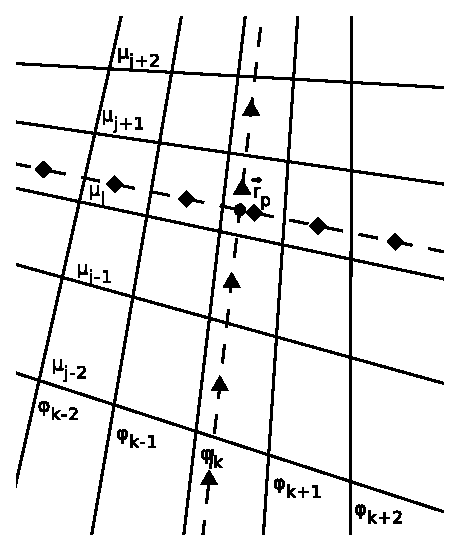
\includegraphics[width=2.5in]{GaussianGeometry.eps}} 
	\vspace*{8pt}
	\caption{Gaussian ray nearest neighbors 
		(front view: \(t_n\) direction not shown).}
	\label{fig:ray_neighbors}
\end{figure}
In all Gaussian beam models, the intensity at the target location is a summation of
contributions from the rays that surround the eigenray target. 
To create a \threeD acoustic field across the wavefront, the new model uses 
independent Gaussian beams in the
\(\mu\) and \(\varphi\) directions and ignores the cross terms. As
illustrated in Fig.~\ref{fig:ray_neighbors} and
Eq.~(\ref{eq:gaussian_sum}), this assumption decomposes the Gaussian ray
contributions to a series of nearest neighbor lines in the \(\mu\) and
\(\varphi\) directions
\begin{equation}
	G(\vec{r}_p) = \left( \sum_{j'=j-J}^{j+J} g_{j'}(\vec{r}_p)\right) 
		\left( \sum_{k'=k-K}^{k+K} g_{k'}(\vec{r}_p)\right) \:,
	\label{eq:gaussian_sum}
\end{equation}
where
\(G(\vec{r}_p)\) is the total Gaussian beam intensity at the eigenray target;
$(j,k)$ are the index numbers of cell containing the eigenray target;
\(g_{j'}\) are the Gaussian beam contributions along depression/elevation direction;
\(g_{k'}\) are the Gaussian beam contributions along the azimuthal direction;
$2J+1$ are the number of significant beams in the depression/elevation direction; and
$2K+1$ are the number of significant beams in the azimuthal direction.

The intensity of each Gaussian beam contribution is a function of the width
of the beam and the distance along the wavefront to the eigenray target,
normalized to the surface area of each beam at the source
\begin{equation}
	g_{j'}(\vec{r}_p) = \frac{ \left( \mu_{j'+1} - \mu_{j'} \right) }
		{\sqrt{2\pi w^2_{j'}}} 
		\: exp \left( - \frac{d^2_{j'}}{2w^2_{j'}} \right) \:,
	\label{eq:gaussian_each1}
\end{equation}
\begin{equation}
	g_{k'}(\vec{r}_p) = \frac{ \left( sin(\mu_{j'+1}) - sin(\mu_{j'}) \right) 
		\left( \varphi_{k'+1} - \varphi_{k'} \right) }
		{\sqrt{2\pi w^2_{k'}}} 
		\: exp \left( - \frac{d^2_{k'}}{2w^2_{k'}} \right) \:,
	\label{eq:gaussian_each2}
\end{equation}
where
\(w_{j'}\) and \(w_{k'}\) are the half-widths of the Gaussian beam (from the cell
center to one edge) in the \(\mu\) and \(\varphi\) directions; and
\(d^2_{j'}\) and \(d^2_{k'}\) are the distance in the \(\mu\) and \(\varphi\)
directions from the Gaussian beam center to the eigenray target. Unlike the \Cerveny, GRAB, and BELLHOP models, which use the ray paths to describe the center of each beam, this new model aligns the ray paths with the edges of the Gaussian beam 
(full-width at half maximum).

Distance terms in the \(\mu\) direction are calculated using the following pattern
\begin{equation}
	L = 2 \: w_j \: \frac{\delta \mu}{\Delta \mu_j} \:,
	\label{eq:gaussian_width1}
\end{equation}
\begin{equation}
	d_j = L - w_j \:,
	\label{eq:gaussian_width2}
\end{equation}
\begin{equation}
	d_{j-1} = L - w_{j-1} \:,
	\label{eq:gaussian_width3}
\end{equation}
\begin{equation}
	d_{j-2} = L + 2 w_{j-1} + w_{j-2} \:,
	\label{eq:gaussian_width4}
\end{equation}
\begin{equation}
	d_{j+1} = L - 2 w_j - w_{j+1} \:,
	\label{eq:gaussian_width5}
\end{equation}
\begin{equation}
	d_{j+2} = L - 2 w_j - w_{j+1} - w_{j+2}
	\label{eq:gaussian_width6}
\end{equation}
where
\(\delta \mu\) is the eigenray offset in depression/elevation angle;
\(\Delta \mu\) is the depression/elevation width of this beam at the source;
\(w_j\) is the width of beam $j$;
and all widths have been interpolated to the time \(t_n+\delta t\).
More distant cells can be supported by adding additional $2w$ terms to
Eqs.~(\ref{eq:gaussian_width4}) and (\ref{eq:gaussian_width6}). The pattern
in the azimuthal direction is similar.

GRAB\cite{Weinberg1996} models the frequency dependent component of the
beamwidth by giving each beam a minimum width
\begin{equation}
  w'_j(f) = max \left( w_j, 2 \pi \lambda \right) \:, 
  \label{eq:weinberg_width}
\end{equation}
where 
\(\lambda\) is the wavelength of the signal being modeled;
\(w_j\) is the cell width of beam $j$, and
\(w'_j(f)\) is the adjusted width of beam $j$.
The \(\lambda\) term can be interpreted as the amount of
evanescent spreading that GRAB expects beams to project into neighboring areas.
In GRAB, Gaussian beams are overlapped by 50\% to reduce fluctuations in the vicinity of the mid-point between rays.\cite{Weinberg1996b}  The number of Gaussian profiles is effectively twice the number of ray paths. 

The new algorithm treats beam width broadening as a convolution between a
frequency dependent Gaussian propagation spread and a second Gaussian that
represents the spatial spreading created by the sampling of the wavefront.
\begin{equation}
	(w'_j(f))^2 = \left( 2 w_j \right)^2 + \left( 2 \pi \lambda \right)^2 \:.
	\label{eq:new_width}
\end{equation}
It manages the 50\% overlap by multiplying the cell width term by two.
Treating the two spreading terms in this way avoids the sudden transitions
inherent in taking a maximum value. Normalizing
Eq.~(\ref{eq:gaussian_each1}) by the combined effect of both spreading
sources conserves energy across the wavefront.

Following the example of GRAB and BELLHOP, this new model uses Pedersen's
challenging n\textsuperscript{2} linear environment to provide an initial
evaluation of propagation loss accuracy.\cite{Pedersen1972}
\begin{equation}
	c(z) = \cfrac{c_0}{\sqrt{1+\cfrac{2 g_0 z}{c_0}}} \:,
	\label{eq:n2_linear}
\end{equation}
where
\(c(z)\) is speed of sound as a function of depth;
\(z\) is depth (positive is down);
\(c_0\) is the speed of sound at the ocean surface (=1550.0~m/s); and
\(g_0\) is the sound speed gradient at the ocean surface
(=1.2~s\textsuperscript{-1}).
Note that this test uses the MKS version of the parameters defined in
Jensen, Kuperman, et. al.\cite{Jensen1994} instead of Pedersen's original
English units. As this test case is defined in ``flat earth'' Cartesian coordinates, a
correction must be applied to Eq.~(\ref{eq:n2_linear})
before it can be used by any model based on a spherical earth\cite{Pekeris1946}
\begin{equation}
	c(r) = \frac{r}{R} \: c(z) \:, 
	\label{eq:n2_correction}
\end{equation}
where
$r$ is the radial distance from the center of curvature;
$R$ is the radius of earth's curvature in this area of operations;
$c(z)$ is the original sound speed; and
$c(r)$ is the modified sound speed.

Fig.~\ref{fig:n2_shallow} plots the coherent propagation loss for this new
model, as a function of range, for a source/receiver depth of 75~m, and
a frequency of 2000 Hz. Target locations are analyzed between 500 and 1000~m
to illustrate the behavior of the model near the edge of the shadow zone at 880~m.
Fig.~\ref{fig:n2_shallow} also plots the corresponding results for the
GRAB model and the Fast Field Program (FFP) wavenumber integration
model.\cite{DiNapoli1980,Brekhovskikh1980} Note that, in all regions, this
implementation of FFP is consistent with an ideal wave equation solution except
for the presence of some minor implementation jitter in the ranges above 880~m.

Prior to the shadow zone, all three models produce similar results. In the
region beyond 840~m, this new approach and GRAB produce values that are
similar to each other, but slightly higher than the theory. Results such as
these lead us to believe that this new model can produce propagation loss
values that are equivalent to standard benchmarks, even though the
formulation of this new model makes significantly different assumptions.

\begin{figure}[th]
	\centerline{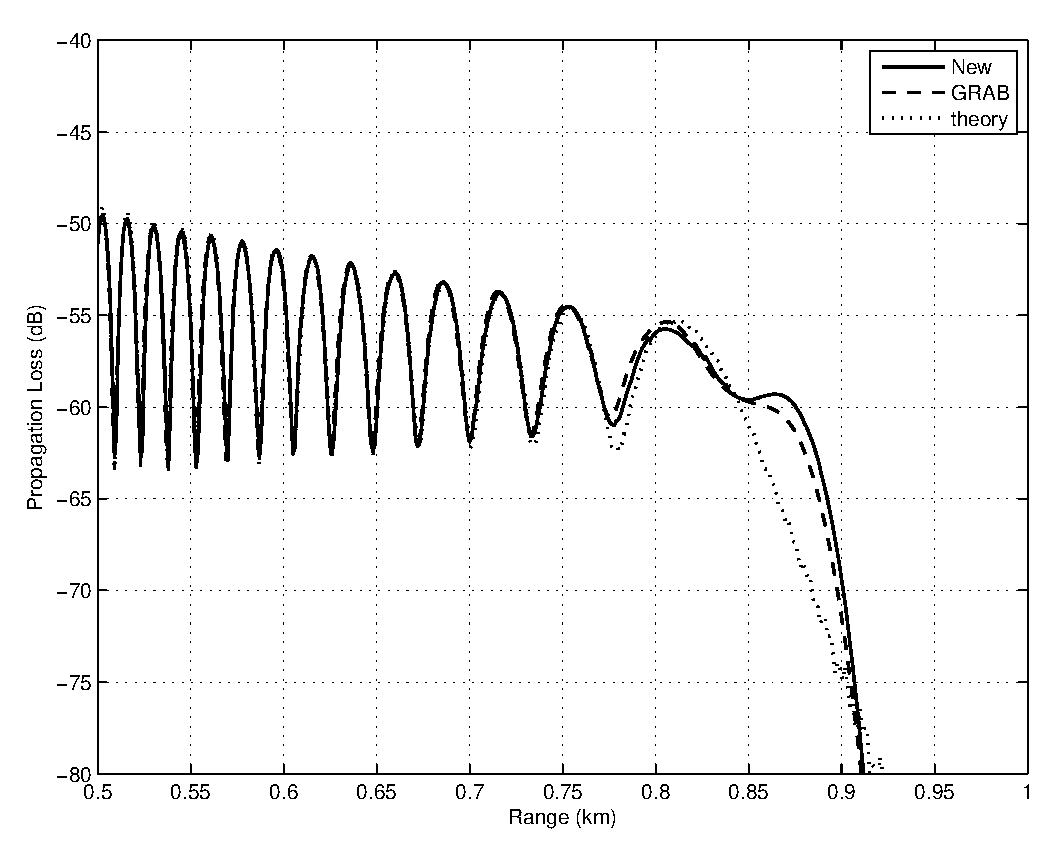
\includegraphics[width=4in]{pedersen_shallow_compare.eps}} 
	\vspace*{8pt}
	\caption{Model comparisons at edge of shadow zone. \label{fig:n2_shallow}}
\end{figure}

\section{Summary}

This paper has derived a new hybrid Gaussian beam model for computing
propagation loss and eigenrays in a \threeD environment. The Gaussian beam
components of this new approach leverage the concepts developed by Weinberg
and Keenan for the GRAB model. However unlike GRAB, which is \twoDxN, this
new algorithm uses HARPO's latitude, longitude, and altitude concept as the
basis for its \threeD propagation environment. Computing the propagation
loss in the same coordinate system as the environmental parameters should
provide this model with a computational speed advantage over other models.
The derivation of this new approach requires the development of new
equations for ray tracing, reflection, eigenray finding, and Gaussian beam
propagation loss. Preliminary tests suggest that these changes have not had
a negative impact on the accuracy of the model. However, more work is still
required to verify and validate this accuracy and to evaluate the new
model's computational efficiency.

\appendix

\section{Derivation of the Ray Equations in Spherical/Time Coordinates}

Ray theory decomposes acoustic waves into surfaces of constant travel time
(\(t\)) from the source (Fig.~\ref{fig:geometry}). The rays are a vector
field that is normal to these surfaces at each point in space, and the route of
these rays through the medium defines the direction of propagation. In the
high frequency limit, spreading loss occurs as the energy of the wavefront
is stretched over increasingly larger areas during propagation. Classic ray
theory uses the change in distance between rays to model the spreading
effects of wavefront propagation.
\begin{figure}[th]
	\centerline{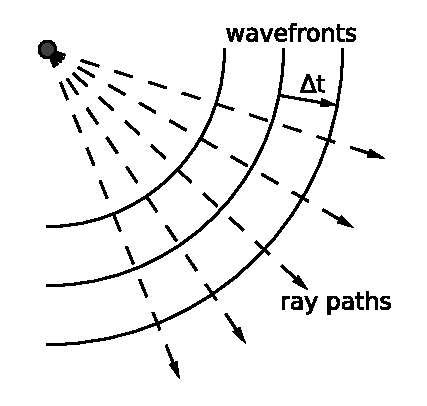
\includegraphics[width=2in]{AcousticRayGeometry.eps}} 
	\vspace*{8pt}
	\caption{Acoustic ray geometry.  \label{fig:geometry}}
\end{figure}
The fundamental equations of ray theory are derived\cite{Jensen1994} by
seeking solutions to the Helmholtz equation (\ref{eq:helmholtz}) in the
form given by Eq.~(\ref{eq:helmholtz_solution})
\begin{equation}
	\nabla^2p + \frac{\omega^2}{c^2(\vec{r})} p(\vec{r}) 
		= -\delta(\vec{r}-\vec{r}_0)
	\label{eq:helmholtz}
\end{equation}
\begin{equation}
	p(\vec{r}) = e^{i \omega t(\vec{r}) } 
		\sum_{j=0}^{\infty} \frac{ A_j(\vec{r}) }{(i\omega)^j} \:.
	\label{eq:helmholtz_solution}
\end{equation}

Equating terms of like order in \(\omega\), yields the infinite sequence of
equations given by Eqs.~(\ref{eq:eikonal}), (\ref{eq:transport}), and
(\ref{eq:diffraction})
\begin{equation}
	O(\omega^2) : \left| \vec{\nabla}t \right|^2 = \frac{1}{c^2(\vec{r})} \:,
	\label{eq:eikonal}
\end{equation}
\begin{equation}
	O(\omega) : 2\vec{\nabla}A_0 \cdot \vec{\nabla}t + (\nabla^2t)A_0 = 0 \:,
	\label{eq:transport}
\end{equation}
\begin{equation}
	O(\omega^{1-j}) : 2\vec{\nabla}A_j \cdot \vec{\nabla}t + (\nabla^2t)A_j 
		= -\nabla^2 A_{j-1} \qquad \text{for j=1,2,...}
	\label{eq:diffraction}
\end{equation}
where 
\(\vec{r}\) is the position coordinate along a ray path;
$c$ is the speed of sound in water; 
$A$ is the wavefront amplitude; and 
$t$ is the travel time along the ray path. 
The eikonal equation (\ref{eq:eikonal}) defines the relationship between
the direction of propagation and the speed of sound in water. The first
transport equation (\ref{eq:transport}) relates the spreading loss of the
acoustic field to the divergence in the propagation direction. The
remaining transport equations (\ref{eq:diffraction}) relate the spreading
loss of the acoustic field to diffraction effects. Eqs.~(\ref{eq:eikonal})
and (\ref{eq:transport}) are an exact solution of the wave equation in the
geometric limit, that is, when the sound speed gradient along the direction
of motion changes slowly compared to the acoustic wavelength. The accuracy
starts to break down at lower frequencies where diffraction becomes a
significant feature of acoustic propagation.

The analytic solution to the eikonal equation (\ref{eq:eikonal}) is
found\cite{Jensen1994} by relating \(\vec{\nabla}t\) to \(\hat{n}\), the
direction of energy propagation along the ray paths
\begin{equation}
	\hat{n} = \frac{d\vec{r}}{ds} = c \vec{\nabla}t \:.
	\label{eq:ray_paths}
\end{equation}

This transforms the eikonal equation into a second order ordinary
differential equation in terms of \(\vec{r}\), $c$, and $s$
\begin{equation}
	\frac{d}{ds} \left( \frac{1}{c} \frac{d\vec{r}}{ds} \right) 
		= -\frac{1}{c^2} \vec{\nabla}c \:.
	\label{eq:ode2}
\end{equation}

This can be reduced to a pair of simultaneous first order equations by
introducing the temporary variable \(\vec{\xi}\)
\begin{equation}
	\frac{d\vec{\xi}}{ds} = -\frac{1}{c^2} \vec{\nabla}c \:,
	\label{eq:dxi_ds}
\end{equation}
\begin{equation}
	\frac{d\vec{r}}{ds} = c \vec{\xi} \:.
	\label{eq:dr_ds}
\end{equation}

This set of equations can be solved using a series of arc length steps
given initial conditions.\cite{Yakowitz1986,Press1992}
Equation~(\ref{eq:dr_ds}) suggests that the temporary variable
\(\vec{\xi}\) is actually the direction of propagation scaled by the speed
of sound, or equivalently, the wave number vector divided by the angular
frequency
\begin{equation}
	\vec{\xi} = \frac{\hat{n}}{c} = \frac{\vec{k}}{\omega} \:,
	\label{eq:n_c}
\end{equation}
where 
\(\vec{k}\) is the acoustic wave number vector; and
\(\omega\) is the angular frequency of the acoustic source.
This definition of \(\vec{\xi}\) allows the system of equations represented
by Eqs.~(\ref{eq:dxi_ds}) and (\ref{eq:dr_ds}) to be initialized with the
position and steering angle for each ray path at the acoustic source.
Note that the steering angle is defined using the depression/elevation (\(\mu\)) and the azimuthal steering (\(\varphi\)) launch angles of each ray relative to the source.  
Marching the simultaneous first order equations (\ref{eq:dxi_ds}) and (\ref{eq:dr_ds}) through steps in arc length then
generates ray paths throughout the water column. The spreading loss of the
wavefront at any point is calculated by measuring the spreading between
adjacent rays. As adjacent rays have different travel times in this
treatment, there is an implicit assumption that propagation loss is being
calculated for a continuous ensonification at a single frequency.

To maintain the phase continuity of the wavefront, the change of
variables defined in Eq.~(\ref{eq:d_ds}) is used to transform the ray
equations into a function of travel time
\begin{equation}
	\frac{d}{ds} = \frac{1}{c} \frac{d}{dt} \:, 
	\label{eq:d_ds}
\end{equation}
\begin{equation}
	\frac{d\vec{\xi}}{dt} = -\frac{1}{c} \vec{\nabla}c \:,
	\label{eq:dxivec_dt}
\end{equation}
\begin{equation}
	\frac{d\vec{r}}{dt} = c^2 \vec{\xi} \:.
	\label{eq:drvec_dt}
\end{equation}

This form of the marching solution computes propagation as a series of
steps in travel time and the phase coherence between rays is preserved at
each step. This form of the ray equation represents a broadband impulse
response of the environment in the high frequency limit. Note that although
the ray paths represented by Eqs.~(\ref{eq:dxivec_dt}) and
(\ref{eq:drvec_dt}) are independent of frequency, the loss along those
paths will include the frequency dependent effects of seawater absorption
and interface reflection.

\begin{figure}[th]
	\centerline{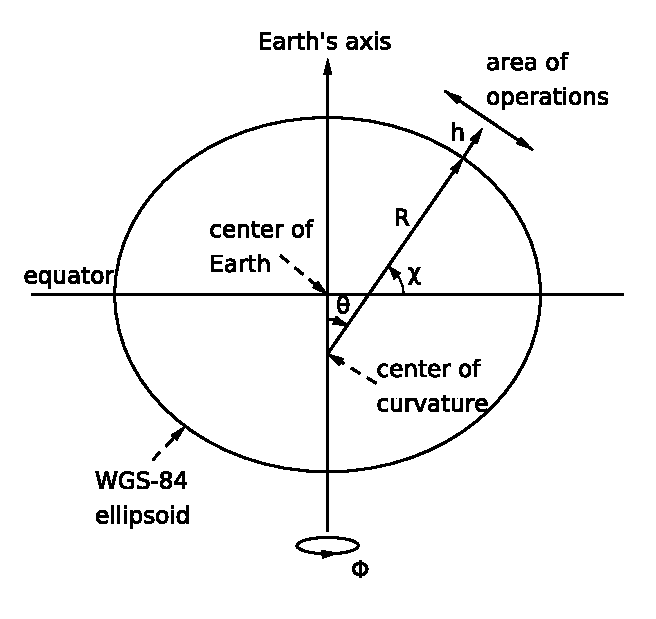
\includegraphics[width=3in]{SphericalEarthCoordinates.eps}} 
	\vspace*{8pt}
	\caption{Spherical earth coordinates.}
	\label{fig:earth}
\end{figure}

This new approach uses the World Geodetic System 1984 (WGS--84)\cite{WGS84} reference ellipse to represent zero altitude worldwide (mean sea level). A
spherical polar coordinate system is constructed within each area of
operations, and its radius is set equal to the WGS--84 radius of curvature
at the center of the area. This coordinate system is illustrated in
Fig.~\ref{fig:earth} 
where 
\(\chi\) is latitude;
\(\phi\) is longitude; 
$h$ is altitude above mean sea level;
$R$ is radius of earth's curvature for the area of operations;
$r$ is distance from the center of curvature (R+h); and 
\(\theta\) is co-latitude (\(90^\circ-\chi\)).

This model defines the average radius of curvature in the area of
operations using a combination of WGS--84 radii in the latitude and
longitude directions\cite{Jones1986}
\begin{equation}
	w^2 \equiv 1 - e^2 cos\chi \:,
	\label{eq:w^2}
\end{equation}
\begin{equation}
	R_\chi = \frac{a(1-e^2)}{w^3} \:,
	\label{eq:R_chi}
\end{equation}
\begin{equation}
	R_\phi = \frac{a}{w} \:,
	\label{eq:R_phi}
\end{equation}
\begin{equation}
	R = \sqrt{ R_\chi R_\phi }
	\label{eq:Rtotal}
\end{equation}
where 
$e$ is the WGS--84 elliptic eccentricity of earth (8.1819190842622x10\textsuperscript{-2});
$a$ is the WGS--84 equatorial radius of the earth (6378137.0~m);
(\(R_\chi\),\(R_\phi\)) are the radii of curvature in the latitude and longitude directions; 
and $R$ is the average radius of curvature in area of operations.  

From these definitions, all locations in the area of operations can be
represented in terms of the spherical polar properties
($r$,\(\theta\),\(\phi\)). The transformation of Eqs.~(\ref{eq:dxivec_dt})
and (\ref{eq:drvec_dt}) into this coordinate system uses the fact that the
ray position only has radial components, while the ray direction has
components in all three dimensions.\footnote{This derivation uses arrows for
vectors with magnitude and direction (such as \(\vec{r}\)), carets for unit
length vectors (such as \(\hat{r}\)), and plain text for magnitude
parameters (such as $r$).}
\begin{equation}
	\vec{r}(t) = r(t) \hat{r}(t) \:,
	\label{eq:spherical1}
\end{equation}
\begin{equation}
	\vec{\xi}(t) = \alpha(t) \hat{r}(t) + \beta(t) \hat{\theta}(t) 
		+ \gamma(t) \hat{\phi}(t) \:,
	\label{eq:spherical2}
\end{equation}
\begin{equation}
	\frac{d\vec{r}}{dt} = \frac{dr}{dt} \hat{r} + r \frac{d\hat{r}}{dt} \:,
	\label{eq:spherical3}
\end{equation}
\begin{equation}
	\frac{d\vec{\xi}}{dt} = \frac{d\alpha}{dt} \hat{r} + \alpha \frac{d\hat{r}}{dt}
	+ \frac{d\beta}{dt} \hat{\theta} + \beta \frac{d\hat{\theta}}{dt}
	+ \frac{d\gamma}{dt} \hat{\phi} + \gamma \frac{d\hat{\phi}}{dt}
\label{eq:spherical4}
\end{equation}
where 
\(\alpha(t)\), \(\beta(t)\), and \(\gamma(t)\) are the radial,
co-latitude, and longitude components of the normalized ray direction.
Note that the unit vectors \(\hat{r}\), \(\hat{\theta}\), and \(\hat{\phi}\) 
in Eqs.~(\ref{eq:spherical3}) and (\ref{eq:spherical4})
change as a function of $r$, \(\theta\),
and \(\phi\). The impact of these derivatives can be understood by casting
them into their Cartesian coordinate equivalents before applying the time
derivative
\begin{equation}
	\hat{r}(t) = sin\theta(t) \: cos\phi(t) \: \hat{i}
		+ sin\theta(t) \: sin\phi(t) \: \hat{j}
		+ cos\theta(t) \: \hat{k} \:,
	\label{eq:rhat}
\end{equation}
\begin{equation}
	\hat{\theta}(t) = cos\theta(t) \: cos\phi(t) \: \hat{i}
		+ cos\theta(t) \: sin\phi(t) \: \hat{j}
		- sin\theta(t) \: \hat{k} \:,
	\label{eq:thetahat}
\end{equation}
\begin{equation}
	\hat{\phi}(t) = - sin\phi(t) \: \hat{i} + cos\phi(t) \: \hat{j} \:.
	\label{eq:phihat}
\end{equation}

The chain rule, when applied to Eqs.~(\ref{eq:rhat}), (\ref{eq:thetahat}),
and (\ref{eq:phihat}) yields the following time derivatives in spherical
coordinates
\begin{equation}
	\frac{d\hat{r}}{dt} = \frac{d\theta}{dt} \hat{\theta} 
		+ sin\theta \frac{d\phi}{dt} \hat{\phi} \:,
	\label{eq:rhat_dt} 
\end{equation}
\begin{equation}
	\frac{d\hat{\theta}}{dt} = - \frac{d\theta}{dt} \hat{r} 
		+ cos\theta \frac{d\phi}{dt} \hat{\phi} \:,
	\label{eq:thetahat_dt}
\end{equation}
\begin{equation}
	\frac{d\hat{\phi}}{dt} = - sin\theta \frac{d\phi}{dt} \hat{r} \:.
	\label{eq:phihat_dt}
\end{equation}

Applying Eqs.~(\ref{eq:rhat_dt}) through (\ref{eq:phihat_dt}) to
Eqs.~(\ref{eq:spherical3}) and (\ref{eq:spherical4}) transforms the ray
tracing equations into spherical earth coordinates
\begin{equation}
	\frac{d\vec{r}}{dt} = \frac{dr}{dt} \hat{r} + r \frac{d\theta}{dt} \hat{\theta} + r sin\theta \frac{d\phi}{dt} \hat{\phi} \:,
	\label{eq:rays_r}
\end{equation}
\begin{equation}
	\begin{split}
		\frac{d\vec{\xi}}{dt} = \left[ \frac{d\alpha}{dt} - \beta \frac{d\theta}{dt} 
			+ \gamma sin\theta \frac{d\phi}{dt} \right] \hat{r}
		  	+ \left[ \frac{d\beta}{dt} + \alpha \frac{d\theta}{dt} 
		  	- \gamma cos\theta \frac{d\phi}{dt} \right] \hat{\theta} \\ 
	  	+ \left[ \frac{d\gamma}{dt} + \left( \alpha sin\theta 
	  	+ \beta cos\theta \right) \frac{d\phi}{dt} \right] \hat{\phi} \:.
	  	\label{eq:rays_xi}
	\end{split}
\end{equation}

Matching terms for \(\hat{r}\), \(\hat{\theta}\), and \(\hat{\phi}\) yields
a system of six first-order, scalar differential equations
\begin{equation}
\frac{dr}{dt} = c^2 \alpha \:,
\label{eq:sixscalar1}
\end{equation}
\begin{equation}
	r \frac{d\theta}{dt} = c^2 \beta \:,
	\label{eq:sixscalar2}
\end{equation}
\begin{equation}
	r sin\theta \frac{d\phi}{dt} = c^2\gamma \:,
	\label{eq:sixscalar3}
\end{equation}
\begin{equation}
	\frac{d\alpha}{dt} - \beta \frac{d\theta}{dt} 
		- \gamma sin\theta \frac{d\phi}{dt} 
		= -\frac{1}{c}\frac{dc}{dr} \:,
	\label{eq:sixscalar4}
\end{equation}
\begin{equation}
	\frac{d\beta}{dt} + \alpha \frac{d\theta}{dt} 
		- \gamma cos\theta \frac{d\phi}{dt} 
		= -\frac{1}{cr}\frac{dc}{d\theta} \:,
	\label{eq:sixscalar5}
\end{equation}
\begin{equation}
	\frac{d\gamma}{dt} + \left( \alpha sin\theta 
		+ \beta cos\theta \right) \frac{d\phi}{dt} 
		= -\frac{1}{cr sin\theta}\frac{dc}{d\phi} \:.
	\label{eq:sixscalar6}
\end{equation}

When Eqs.~(\ref{eq:sixscalar1}) though (\ref{eq:sixscalar3}) are plugged
into Eqs.~(\ref{eq:sixscalar4}) though (\ref{eq:sixscalar6}), the system is
reduced to a state where all of the coordinate derivatives appear only once
\begin{equation}
	\frac{dr}{dt} = c^2 \alpha \:,
\end{equation}
\begin{equation}
	\frac{d\theta}{dt} = \frac{c^2 \beta}{r} \:,
\end{equation}
\begin{equation}
	\frac{d\phi}{dt} = \frac{c^2\gamma}{r sin\theta} \:,
\end{equation}
\begin{equation}
	\frac{d\alpha}{dt} = -\frac{1}{c}\frac{dc}{dr} 
		+ \frac{c^2}{r}\left( \beta^2 + \gamma^2 \right) \:,
\end{equation}
\begin{equation}
	\frac{d\beta}{dt} = -\frac{1}{cr}\frac{dc}{d\theta} 
		- \frac{c^2 \alpha \beta}{r} + \gamma^2 cot\theta \:,
\end{equation}
\begin{equation}
	\frac{d\gamma}{dt} = -\frac{1}{cr sin\theta}\frac{dc}{d\phi} 
		- \frac{c^2 \gamma}{r} \left( \alpha + \beta cot\theta \right) \:.
\end{equation}
These are the ray equations in spherical/time coordinates.

\section*{Acknowledgments}

This paper was developed as part of Sean Reilly's PhD studies at the Ocean
Engineering Department of the University of Rhode Island, under the
direction of Dr. Gopu Potty and Dr. James Miller. Testing an productization
of this model were funded by the High Fidelity Active Sonar Training
(HiFAST) Project at the U.S. Office of Naval Research. The theory for
reflection from a \threeD slope was developed by Mr. Michael Goodrich, who
also made significant contributions to the development of early test cases
for this model. The authors would also like to thank Dr. Charles Holland
(ARL/PS) for his editorial help in preparing this manuscript.

\begin{thebibliography}{0}
\bibitem{Baxley2000} P. A. Baxley, H. Bucker, M. B. Porter, Comparison of
Beam Tracing Algorithms, {\it Proceedings of the Fifth European Conference
on Underwater Acoustics (ECUA)} {2000}.

\bibitem{Weinberg1996} H. Weinberg, R. E. Keenan, Gaussian ray bundles for
modeling high-frequency propagation loss under shallow-water conditions,
{\it J. Acoust. Soc. Amer.} {\bf 100} (1996) 1421.

\bibitem{GRAB2008} Software Requirements Specification/Software Design
Description and Software Test Description for the Oceanographic and
Atmospheric Master Library Navy Standard Comprehensive Acoustic System
Simulation Model Version 4.2A, {\it Naval Meteorology and Oceanography
Command Report OAML-SRS-SDD-STD-83D} (2008).

\bibitem{Cerveny1982} V. \Cerveny, M. M. Popov, and I. P\v{s}enc\'{i}k, Computation
of wave fields in inhomogeneous media - Gaussian beam approach, {\it
Geophys. J. R. Astron. Soc.} {\bf 70} (1982) 109.

\bibitem{Porter1994} M. B. Porter, Y. C. Liu, Finite Element Ray Tracing, 
{\it International Conference on Theoretical and Computational Acoustics (ICTCA)} Volume 2 (1994) 947.

\bibitem{Porter1987} M. B. Porter, H. P. Bucker, Gaussian beam tracing for
computing ocean acoustic fields, {\it J. Acoust. Soc. Amer.} {\bf 93}
(1987) 1349.

\bibitem{Jones1986} R. M. Jones, J.P. Riley, T.M. Georges, HARPO: A
Versatile Three-Dimensional Hamiltonian Ray-Tracing Program for Acoustics
Waves in an Ocean with Irregular Bottom, {\it National Oceanic and
Atmospheric Administration (NOAA) Report}, (1986).

\bibitem{Yakowitz1986} Yakowitz and Szidarovszky, An Introduction to
Numerical Computation (Macmillan Publishing, New York, 1986) pp. 306-311.

\bibitem{Press1992} W. Press, S. Teukolsky, W. Vetterling, B. Flannery,
Numerical Recipes in C (Cambridge University Press, New York, 1992), pp
747-752.

\bibitem{ETOPO1} ETOPO1v2 Global Gridded 2-minute Database, National
Geophysical Data Center, National Oceanic and Atmospheric Administration,
U.S. Dept. of Commerce, http://www.ngdc.noaa.gov/mgg/global/ETOPO1.html.

\bibitem{Sturm2008} F. Sturm, S. Ivansson, Y. M. Jiang, N. R. Chapman,
Numerical investigation of out-of-plane sound propagation in a shallow
water experiment, {\it J.~Acoust. Soc. Amer.} {\bf 124} (2008) pp. 341-346.

\bibitem{Sinnott1984} R. W. Sinnott, Virtues of the Haversine, {\it Sky and
Telescope} {\bf 68} (1984) 159.

\bibitem{Weinberg1996b} H. Weinberg, R. E. Keenan, Gaussian ray bundles for
modeling high-frequency propagation loss under shallow-water conditions, 
NUWC-NPT Technical Report 10,568 (1996).

\bibitem{Pedersen1972} M. A. Pedersen, D. F. Gordon, Normal-Mode and Ray
Theory Applied to Underwater Acoustic conditions of Extreme Downward
Refraction, {\it J. Acoust. Soc. Amer.} {\bf 51} (1972) 323.

\bibitem{Pekeris1946} C. L. Pekeris, Accuracy of the Earth-Flattening Approximation in the Theory of Microwave Propagation, {\it Phys. Rev.} {\bf 70} (1943).

\bibitem{DiNapoli1980} F. R. DiNapoli, R. L. Deavenport, Theoretical and
numerical Green's function field solution in a plane multilayered medium,
{\it J. Acoust. Soc. Amer.} {\bf 67} (1980).

\bibitem{Brekhovskikh1980} L. M. Brekhovskikh, Waves in Layered Media
(Academic Press Inc., New York, 1980), 2nd Edition, Section 54.

\bibitem{Jensen1994} F. B. Jensen, W. A. Kuperman, M. B. Porter, and H.
Schmidt, Computational Ocean Acoustics (American Institute of Physics
Press, New York, 1994) pp. 150-153.

\bibitem{WGS84} WGS 84 Implementation Manual, Version 2.4, {\it European
Organization for the Safety of Air Navigation, and the Institute of Geodesy
and Navigation}, (1998).

\end{thebibliography}
\end{document}

